\documentclass[tikz,border=2pt]{standalone}
\usepackage{amsmath,amssymb}
\usepackage{tikz}
\usetikzlibrary{arrows.meta}

\begin{document}
% S = {1/n : n >= 1}: every number <= 0 is a lower bound; the greatest of them, inf S = 0,
% is not an element of S.
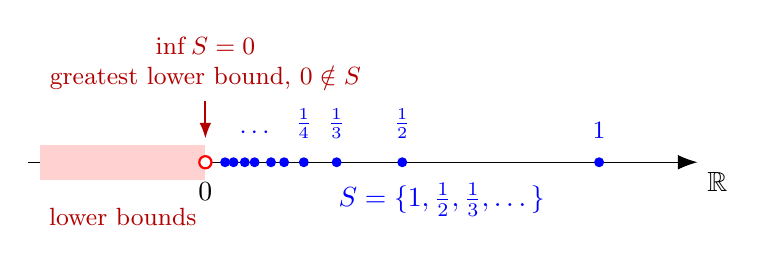
\begin{tikzpicture}[x=5cm]
	\draw[-{Latex[length=2.5mm]}] (-0.45,0) -- (1.25,0) node[below right] {$\mathbb{R}$};
	\fill[red!18] (-0.42,-0.22) rectangle (0,0.22);
	\foreach \n in {1,2,3,4,5,6,8,10,14,20} {\fill[blue] ({1/\n},0) circle (1.8pt);}
	\node[blue, above=5pt, font=\small] at (1,0) {$1$};
	\node[blue, above=5pt, font=\small] at (0.5,0) {$\tfrac12$};
	\node[blue, above=5pt, font=\small] at (0.333,0) {$\tfrac13$};
	\node[blue, above=5pt, font=\small] at (0.25,0) {$\tfrac14$};
	\node[blue, above=5pt, font=\small] at (0.13,0) {$\cdots$};
	\draw[red, thick, fill=white] (0,0) circle (2.2pt);
	\node[below=4pt] at (0,0) {$0$};
	\node[blue, below=4pt] at (0.6,0) {$S=\{1,\tfrac12,\tfrac13,\dots\}$};
	\node[red!70!black, below=13pt, font=\small] at (-0.21,0) {lower bounds};
	\draw[-{Latex[length=2mm]}, red!70!black, thick] (0,0.78) -- (0,0.3);
	\node[red!70!black, above, font=\small, align=center] at (0,0.8) {$\inf S=0$\\ greatest lower bound, $0\notin S$};
\end{tikzpicture}
\end{document}
